\headline{{\textbf{\Large\sffamily The Top Chop:}}\\
          {\textbf{\large\sffamily The Tree of the Month Contest}}}
\label{2025-04-contest}
\noindent
The April gathering of the Twickenham Bonsai Club proved yet again that our members are brimming with creativity and a deep\--rooted love for bonsai.
With the theme \textit{``Juniper, Cypress, or Hemlock,''} the room was bristling with needle\--textured foliage, elegant silhouettes, and resinous charm.
From cascading junipers to rugged sabinas, the display offered a captivating insight into the expressive potential of these much\--loved conifers.
Every tree told a story, whether of windswept mountaintops or quiet refinement in a backyard pot.

For any newcomers or those needing a refresher, here's how the contest works: each member may present one tree per month (novice members may present more, though only the best scoring tree will count toward their annual ranking).
All trees are judged by the attending members---excluding the owner---who score each entry from 1 to 3 marks in four distinct categories: trunk/branches, foliage, pot/container, and overall presentation as it aligns with the month's theme.
This gives a maximum of 12 points per judge per tree, ensuring a well\--rounded and thoughtful evaluation process that celebrates both technical execution and creative vision.

\begin{figure*}[!p]
\centering
\begin{minipage}[b]{.29\textwidth}
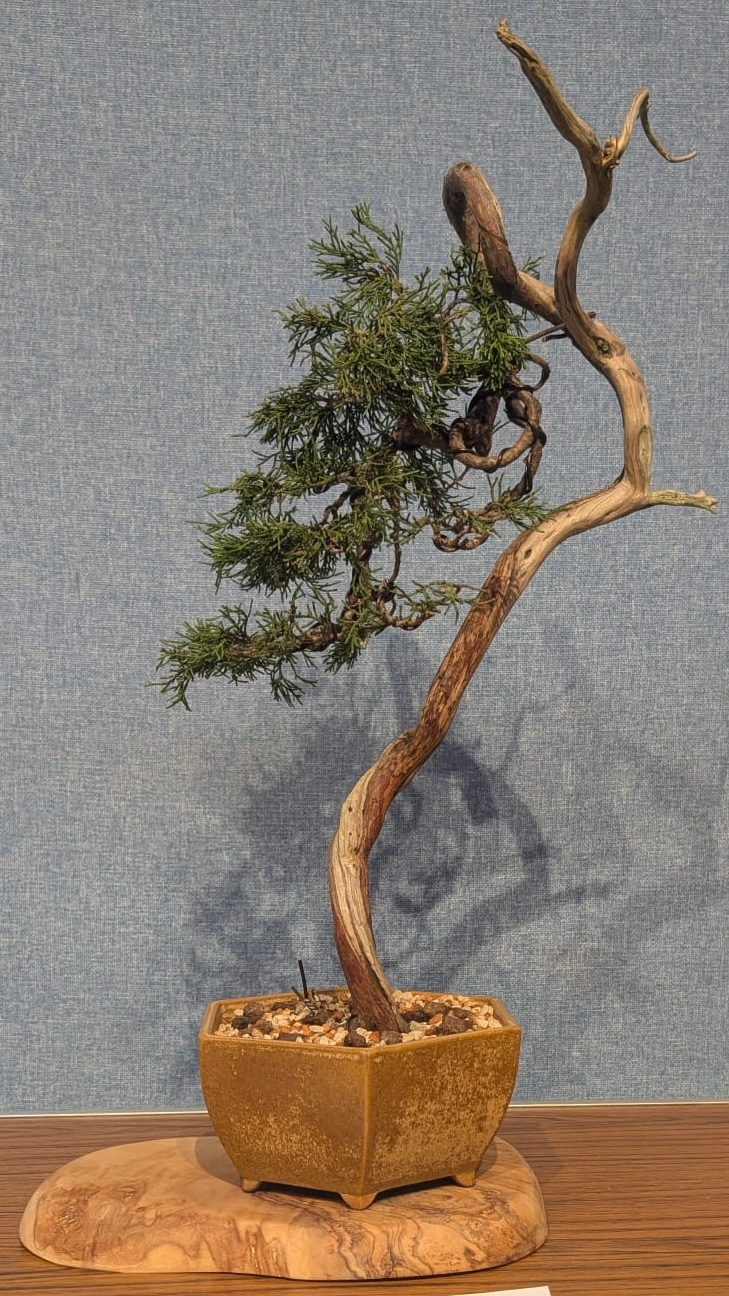
\includegraphics[width=1.0\textwidth]{2025_04/res/contest_tree_04}
\centerline{\emph{Brendan's Bunjin Sabina Juniper.}}
\end{minipage}\qquad
\begin{minipage}[b]{.29\textwidth}
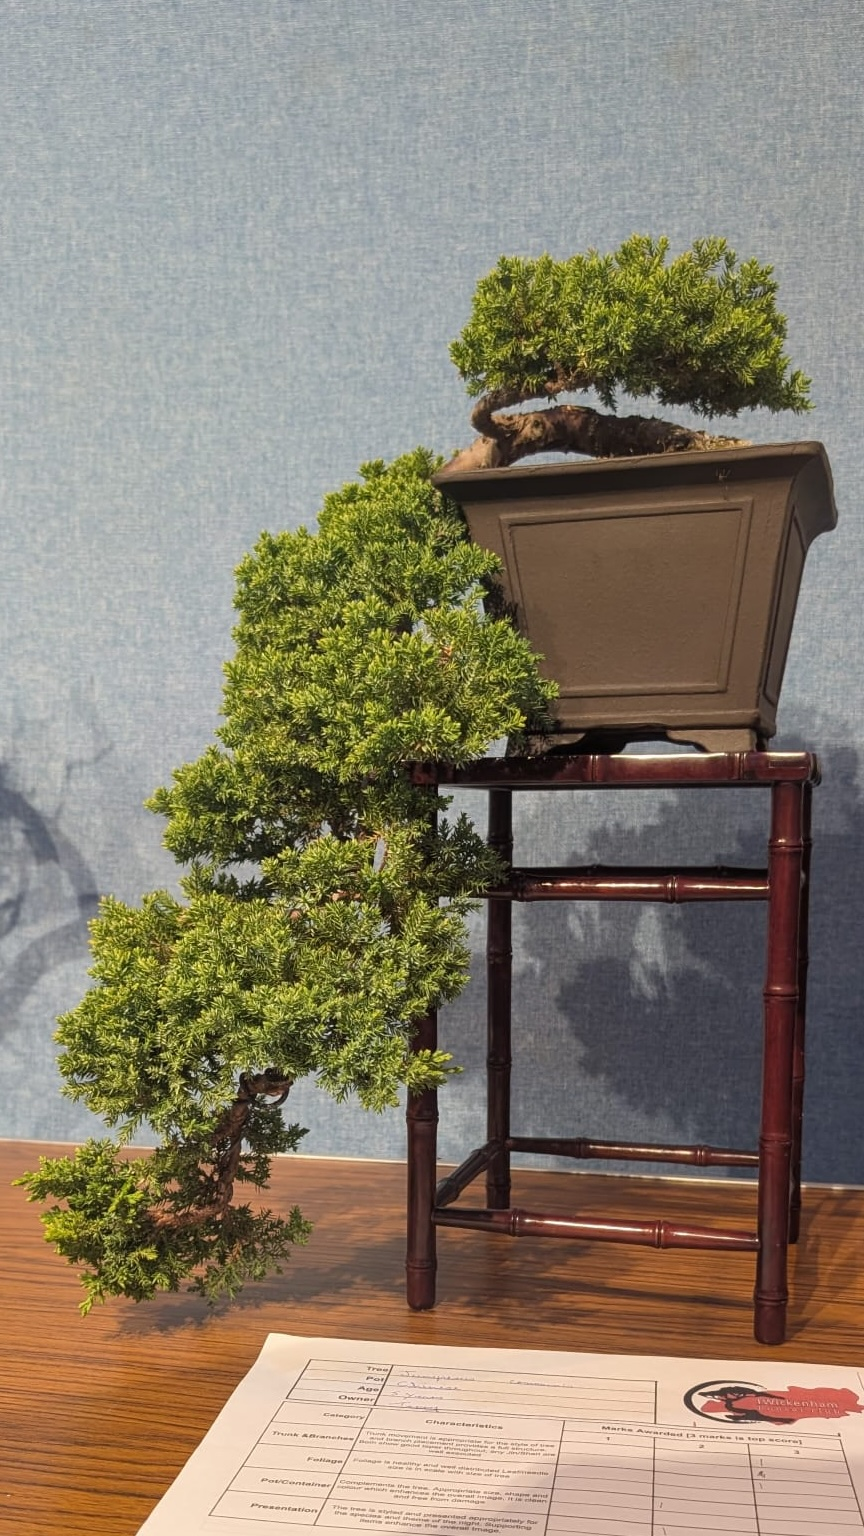
\includegraphics[width=1.0\textwidth]{2025_04/res/contest_tree_05}
\centerline{\emph{Terry's Cascading Procumbens.}}
\end{minipage}\qquad
\begin{minipage}[b]{.29\textwidth}
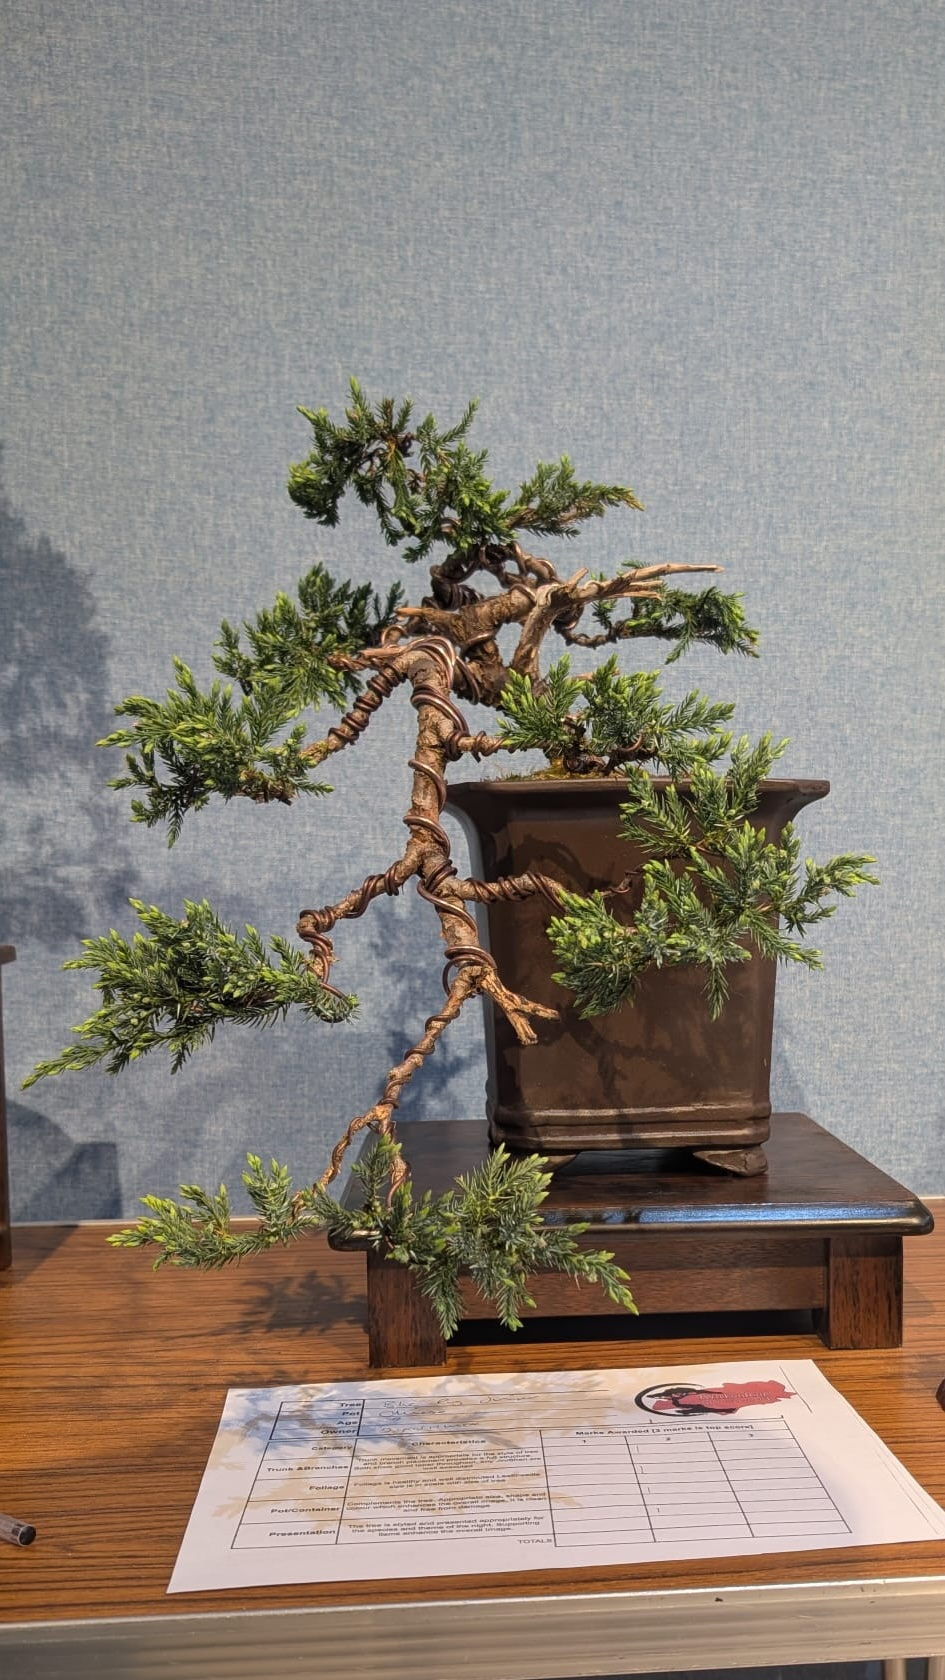
\includegraphics[width=1.0\textwidth]{2025_04/res/contest_tree_06}
\centerline{\emph{David's Semi\--Cascade Juniper.}}
\end{minipage}

\medskip
\begin{minipage}[b]{.29\textwidth}
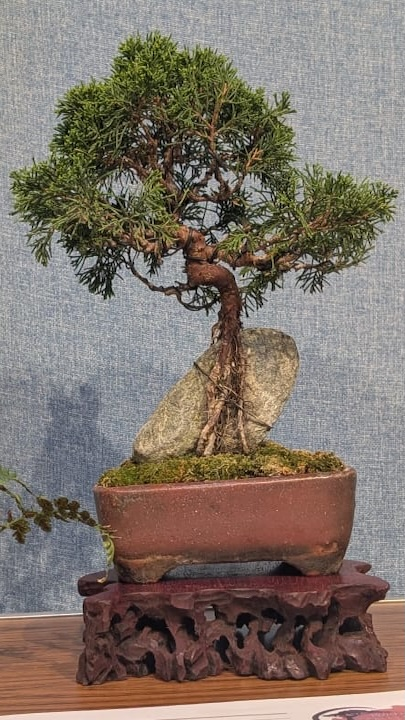
\includegraphics[width=1.0\textwidth]{2025_04/res/contest_tree_03}
\centerline{\emph{Rory's Root\--Over\--Rock Itoigawa.}}
\end{minipage}\qquad
\begin{minipage}[b]{.29\textwidth}
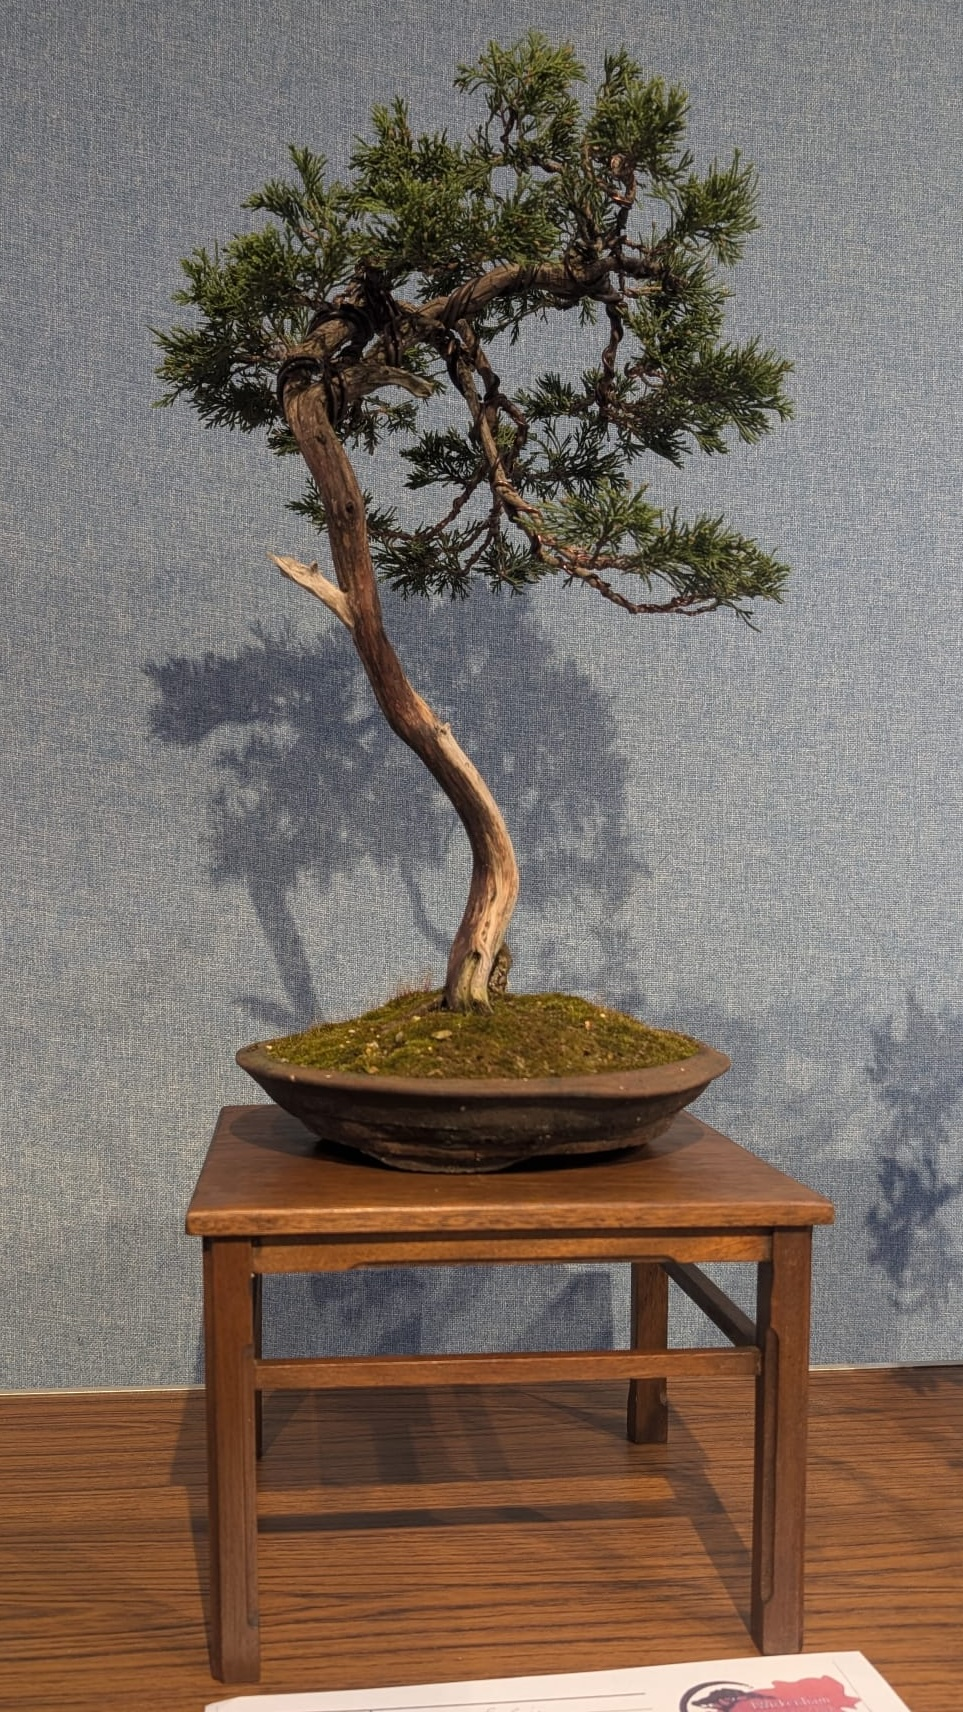
\includegraphics[width=1.0\textwidth]{2025_04/res/contest_tree_01}
\centerline{\emph{Tony's Bunjin Sabina Juniper.}}
\end{minipage}\qquad
\begin{minipage}[b]{.29\textwidth}
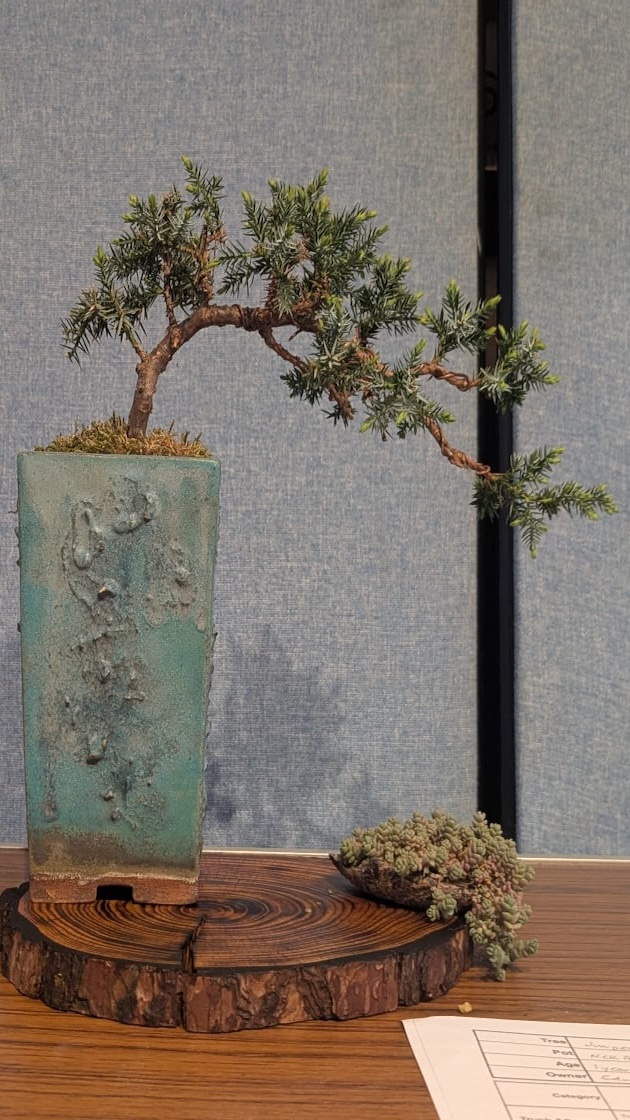
\includegraphics[width=1.0\textwidth]{2025_04/res/contest_tree_02}
\centerline{\emph{Edward's Semi\--Cascade Juniper.}}
\end{minipage}
\end{figure*}

\topic{Tree of the Month}
\noindent 
The \textit{Tree of the Month} category saw an inspiring collection of junipers this April, with each tree reflecting a unique take on the theme.
Here are the results, sorted by points received:

\begin{enumerate}
    \item \textbf{Brendan Gibbs}' venerable sabina juniper (\textit{Juniperus Sabina}, 125 points) --- A soaring bunjin masterpiece, its slender form alive with jins and shari, whispering of windswept cliffs, poised in a pot as refined as its artistry.

    \item \textbf{Terry Wilson}'s expressive juniper (\textit{Juniperus Chinensis}, 122 points) --- A cascading juniper, lush and daring: its curves plunge like a waterfall over cliffs, anchored by a masculine pot, ruling the valley from its stand.

    \item \textbf{David Fishwick}'s low\--growing blue rug juniper (\textit{Juniperus Horizontalis}, 120 points) --- A silver\--blue semi\--cascade, its muscular pads sweeping left and right down the slope like arms embracing the earth from its bold pot.

    \item \textbf{Rory Campbell}'s graceful itoigawa juniper (\textit{Juniperus Chinensis 'Itoigawa'}, 103 points) --- A twisty juniper clinging to its towering rock, roots gripping stone above a \textit{shibui} pot, nature's sculpture of delicate foliage and crisp lines.

    \item \textbf{Tony Ulatowski}'s powerful sabina juniper (\textit{Juniperus Sabina}, 103 points) --- A towering literati with feminine grace, its shari and jin whispering stories from the trunk's base: charismatic yet harmonious.

    \item \textbf{Edward Mason}'s compact juniper (\textit{Juniperus Squamata}, 99 points) --- A promising semi\--cascading tree with lovely texture and a strong foundation, clearly reflecting the artist's growing skill and dedication.
\end{enumerate}

\noindent 
\textbf{Brendan Gibbs} takes the title of \textit{Tree of the Month for April 2025} with his dramatic sabina juniper --- a well\--deserved congratulations!

\topic{Novice Tree of the Month}
\noindent 
The \textit{Novice Tree of the Month} category offered another glimpse into the future of our club, with fresh talent and enthusiasm on full display.
This month's entries were few but full of character.
Results below, sorted by points:

\begin{enumerate}
    \item \textbf{Grant Kinnard}'s crisp European larch (\textit{Larix Decidua}, 97 points) --- A vibrant clump\--style composition, with weathered uros, crowned by lush foliage casting dappled shade over a resting mud\--man; a confident and refined piece that charmed the judges.

    \item \textbf{Riz Mirza}'s bold blue atlas juniper (\textit{Juniperus Virginiana 'Blue Atlas'}, 53 points) --- A lively specimen with vibrant foliage and an energetic cascading posture, promising great potential with future refinement.

    \item \textbf{Paul Raubusch}'s quirky horse chestnut (\textit{Aesculus Hippocastanum}, 44 points) --- A rare sight on the bonsai bench, this creative choice brought miniaturised broad leaves and a playful charm to the table.
\end{enumerate}

\begin{figure*}[p]
\centering
\begin{minipage}[b]{.60\textwidth}
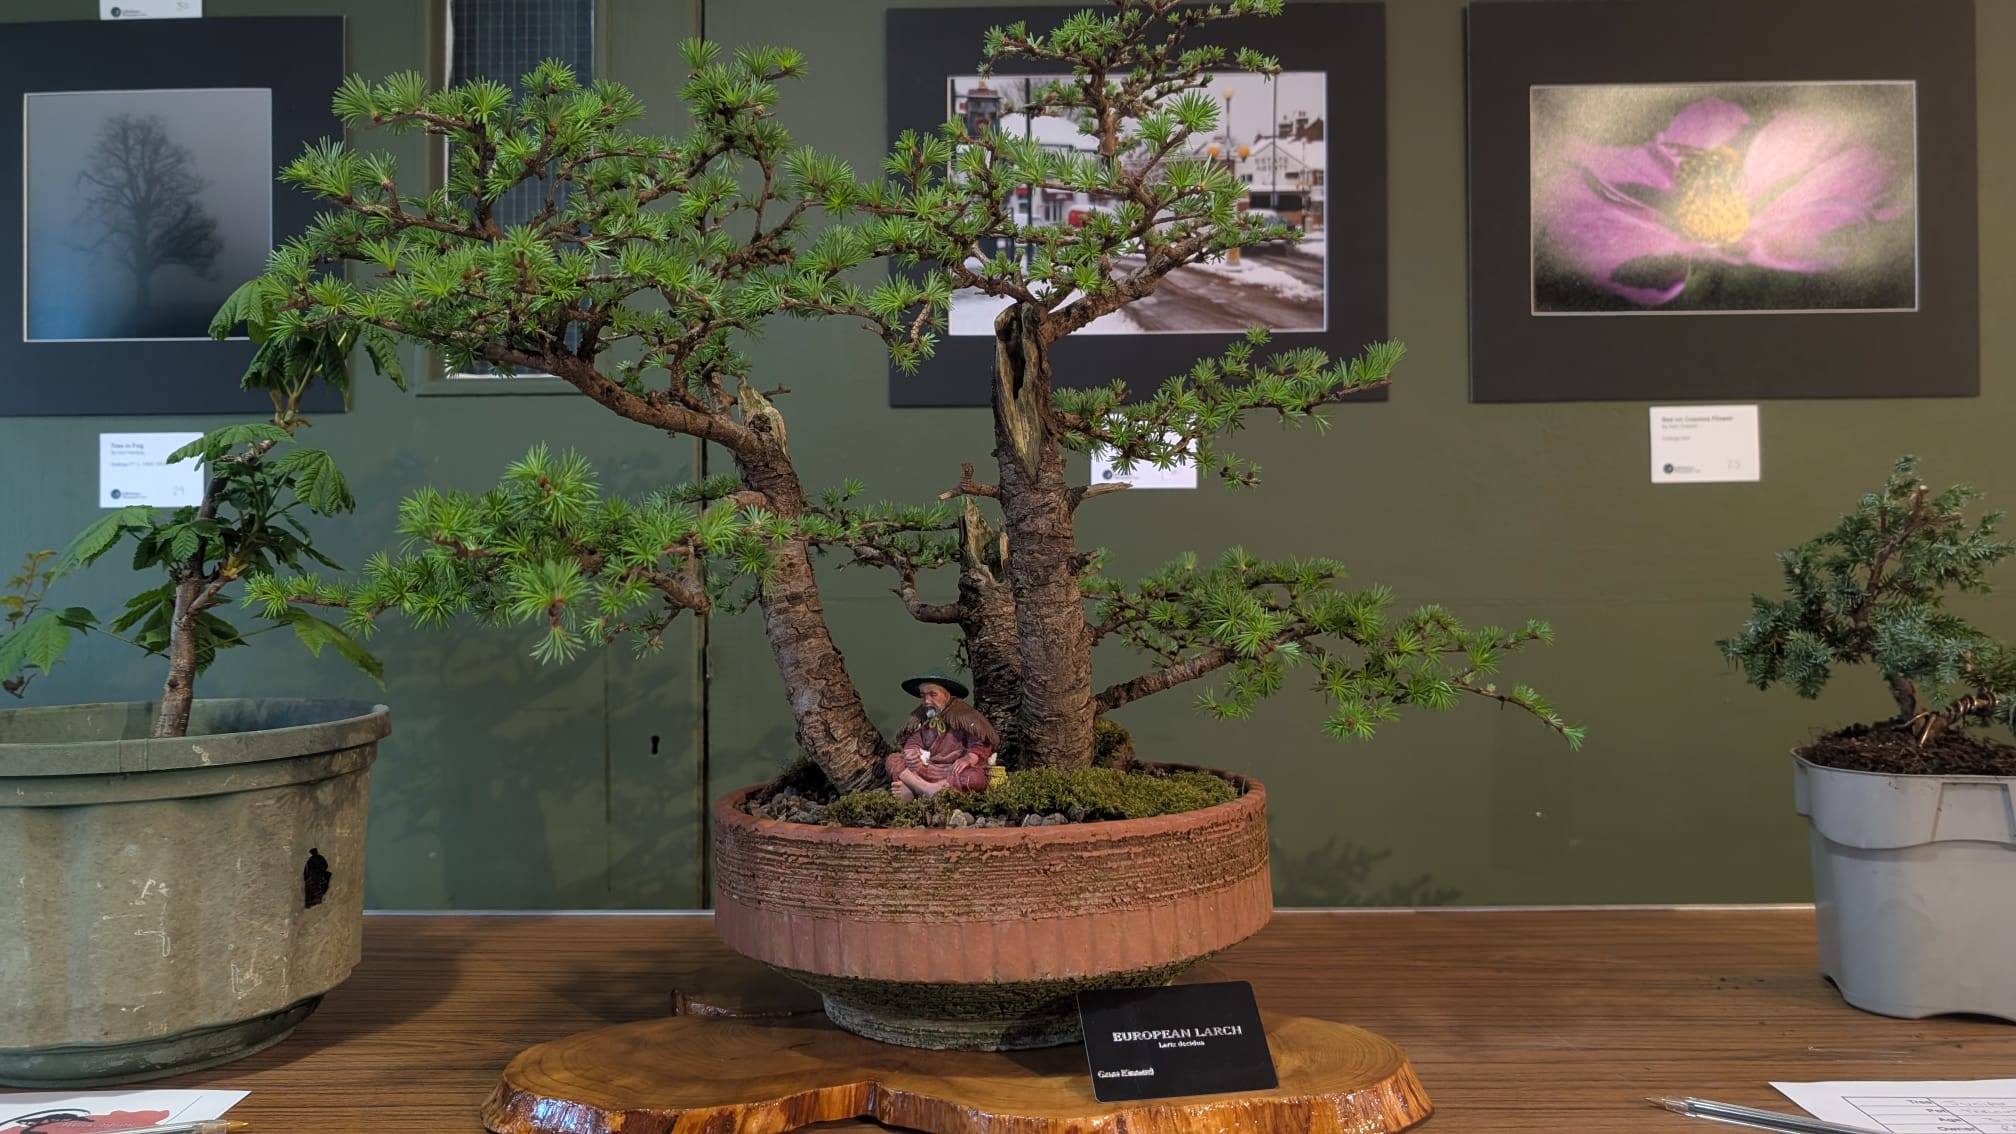
\includegraphics[width=1.0\textwidth]{2025_04/res/contest_novice_02}
\centerline{\emph{Grant's Novice European Larch.}}
\end{minipage}

\medskip
\begin{minipage}[b]{.60\textwidth}
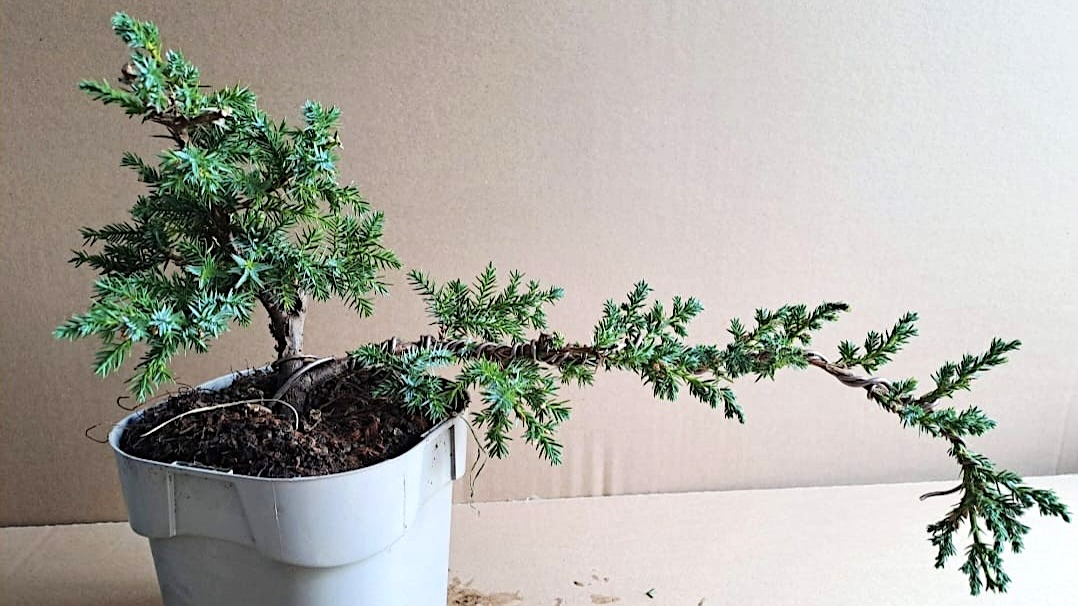
\includegraphics[width=1.0\textwidth]{2025_04/res/contest_novice_03}
\centerline{\emph{Riz's Novice Blue Atlas Juniper.}}
\end{minipage}

\medskip
\begin{minipage}[b]{.60\textwidth}
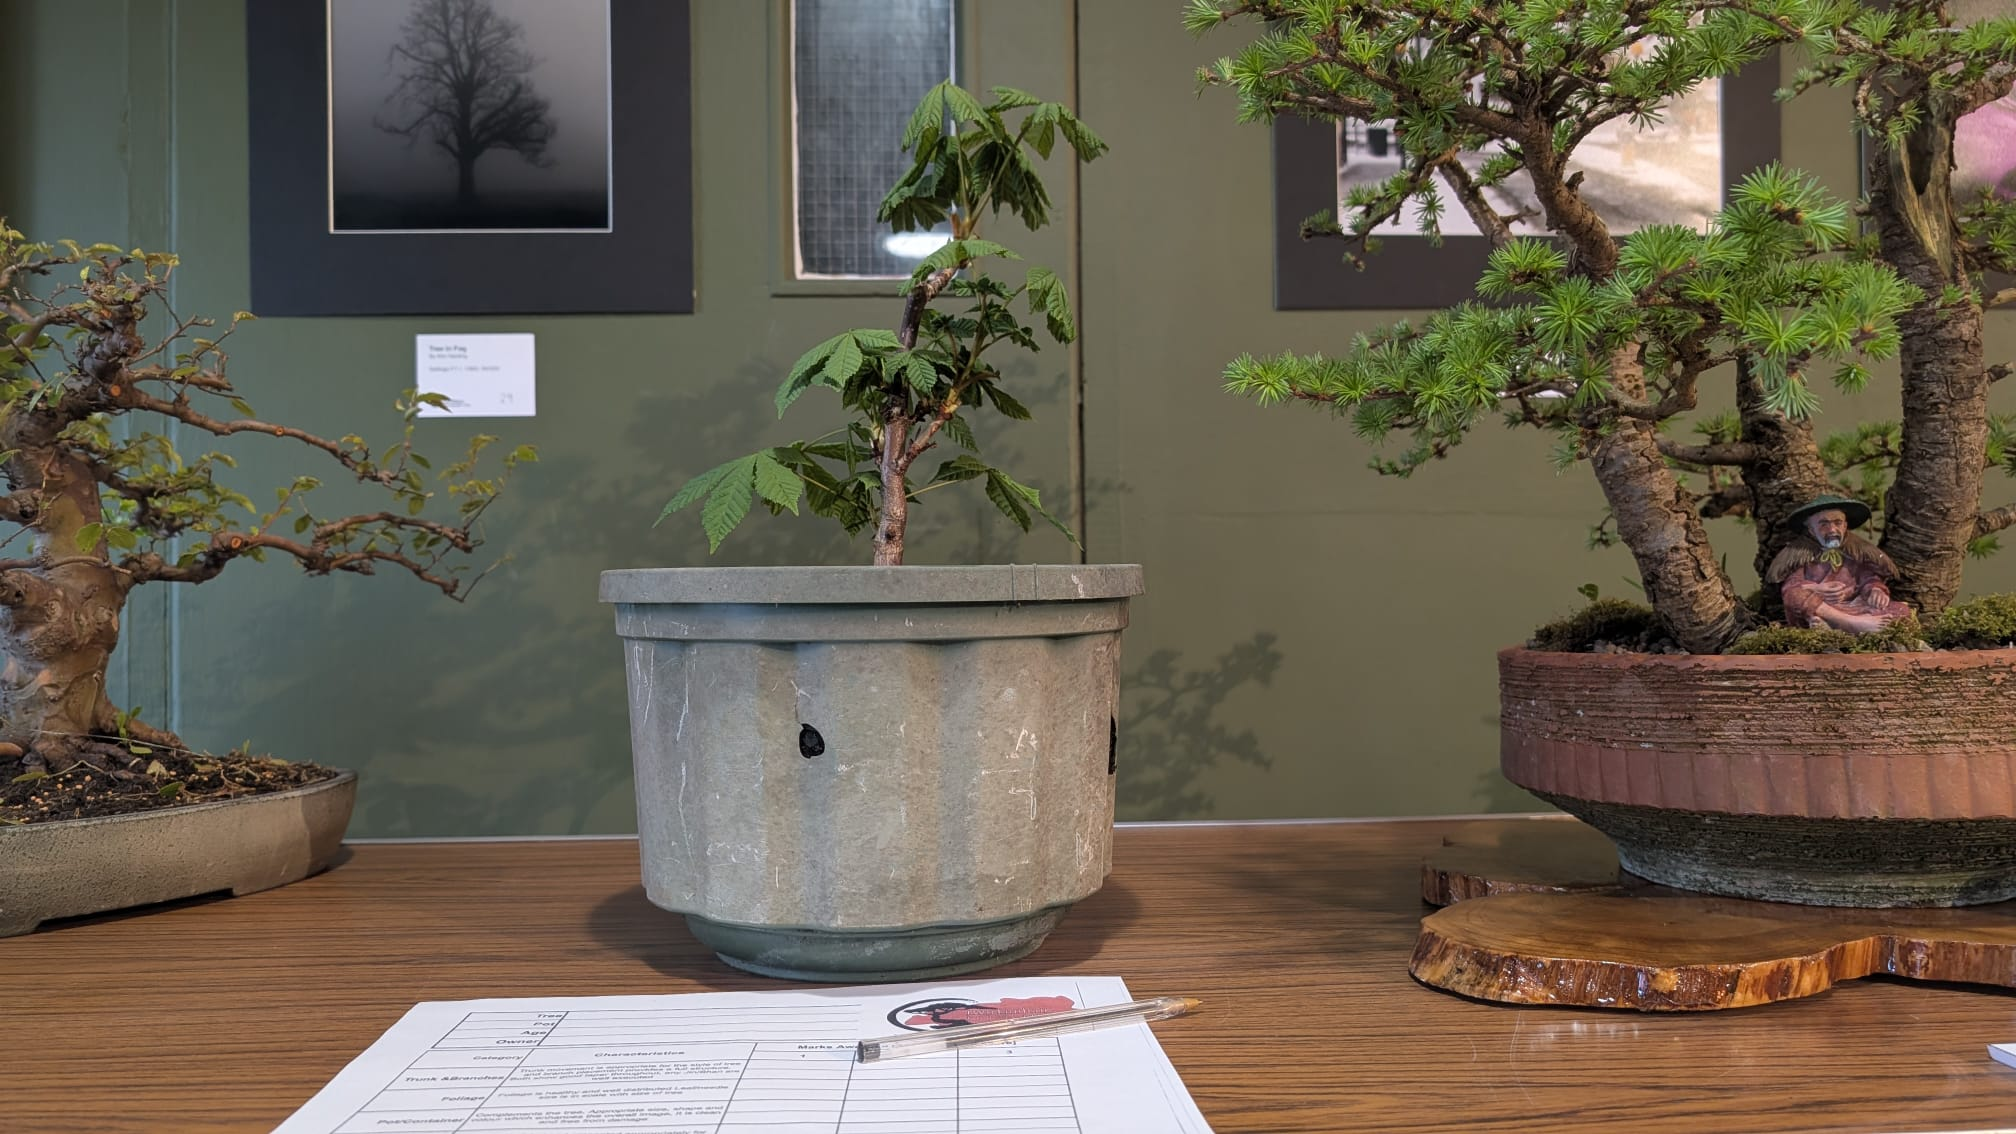
\includegraphics[width=1.0\textwidth]{2025_04/res/contest_novice_01}
\centerline{\emph{Paul's Novice Horse Chestnut.}}
\end{minipage}
\end{figure*}

\noindent
\textit{\textbf{As always, novice members may present multiple trees, but only their highest scoring tree counts toward their end\--of\--year ranking.}}

\medskip
\textbf{Grant Kinnard} is this month's winner of the \textit{Novice Tree of the Month for April 2025} --- fantastic work and congratulations!

\begin{center}
    $\cdots$
\end{center}

\noindent
This month's entries demonstrated just how diverse and dramatic coniferous species can be in the world of bonsai. From weather\--beaten trunks to fine textured foliage, each tree added a different voice to the chorus.
It's this diversity of vision and commitment to craft that keeps our community vibrant and ever\--growing.

Looking ahead, next month's theme is \textit{``Any Flowering Tree''}---share your blossoming bonsai!
As a fun addition, members may also bring \textit{one} \textit{``Mame --- anything under 6 inches''} (measured from the bottom of the pot).
These tiny trees won't be judged, but if the format proves popular, it may become a featured theme next year!

Until then, keep those shears sharp and those trees thriving --- and as always, happy bonsai\--ing!
\closearticle
\columnbreak
